\documentclass[a0paper,portrait]{tikzposter}

\usepackage[utf8]{inputenc}
\usepackage[T1]{fontenc}
\usepackage{lmodern}
\usepackage{microtype}
\usepackage{amsmath,amssymb}
\usepackage{graphicx}
\usepackage{booktabs}
\usepackage{tabularx}
\usepackage{array}
\usepackage{xcolor}
\usepackage{multicol}
\usepackage{enumitem}
\usepackage{relsize}

\graphicspath{{../results/presentation/}{../results/}}

\definecolor{DeepNavy}{HTML}{0B1F3A}
\definecolor{Photon}{HTML}{007C89}
\definecolor{Mist}{HTML}{EEF6F6}
\definecolor{Ink}{HTML}{1F2937}
\definecolor{Amber}{HTML}{D97706}

\setlist[itemize]{nosep,leftmargin=*}
\setlist[enumerate]{nosep,leftmargin=*}

\newcommand{\pjbit}{pJ/bit}
\newcommand{\tbps}{Tb/s}

\definecolorpalette{posterpalette}{
    \definecolor{colorOne}{named}{DeepNavy}
    \definecolor{colorTwo}{named}{Photon}
    \definecolor{colorThree}{named}{Mist}
}
\usecolorpalette{posterpalette}
\usetheme{Simple}
\useblockstyle{Default}
\usetitlestyle{Filled}
\colorlet{blocktitlebgcolor}{DeepNavy}
\colorlet{blocktitlefgcolor}{white}
\colorlet{blockbodybgcolor}{white}
\colorlet{blockbodyfgcolor}{Ink}
\colorlet{notebgcolor}{Mist}
\colorlet{notefgcolor}{Ink}
\colorlet{backgroundcolor}{white}

\title{\parbox{0.92\linewidth}{\centering Topology-Aware Mapping for Photonic Interconnects \\ in TPU-Class LLM Accelerators}}
\author{Pranav Sitaraman \quad \textbullet \quad Simone Surdi}
\institute{MIT 6.5930 / Hardware Architectures for Deep Learning \quad \textbullet \quad Spring 2026 \quad \textbullet \quad Project 12: Evaluate a New Technology}
\titlegraphic{}

\settitle{
\centering
\vbox{\@titlegraphic}\vskip-1ex
{\bfseries\color{white}\Huge \@title}\vskip0.6ex
{\color{white}\large \@author}\vskip0.3ex
{\color{white}\normalsize \@institute}
}

\begin{document}

\maketitle

% Row 1: motivation | underlying principles (2 cols wide)
\begin{columns}
\column{0.32}
\block{1. Motivation}{
\textbf{Why photonic interconnect for TPU pods?} Modern LLM systems
are limited not by matrix-multiply throughput but by the cost of
moving activations, KV-cache state, expert tokens, gradients, and
shared weights between chips. TPU v5p and Ironwood/TPU7x are
organised around high-radix ICI exactly for this reason. Co-packaged
photonics changes \emph{four} interconnect properties at once:
\begin{itemize}
\item Energy/bit drops 3--5$\times$ (10~\pjbit{} $\to$ 3.2/1.9~\pjbit{}).
\item Bandwidth grows 4--70$\times$ (0.8~\tbps{} $\to$ 57.3~\tbps{}).
\item Topology can become a flat switched fabric, not a multi-hop torus.
\item Hardware multicast replaces $N$ unicasts.
\end{itemize}
\textbf{Research question.} Is photonic interconnect a constant-factor
link substitution, or does it change \emph{how a TPU pod should be
mapped and scheduled} for LLM workloads?
Following 6.5930's mapping formalism (partitioning + dataflow + tile
sizing), we separate intra-chip mapping from cluster-level
distributed schedule and ask which layer the gain actually lives in.
}

\column{0.68}
\block{2. Underlying Principles}{
\begin{minipage}[t]{0.62\linewidth}
\textbf{Modeling stack: four layers.}
\begin{enumerate}
\item \textbf{Workload (einsum).} \texttt{single\_matmul.yaml}:
$O_{m,n}=\sum_k A_{m,k}W_{k,n}$ with rank sizes per LLM stage.
\item \textbf{Architecture.}
\texttt{tpu\_lightmatter\_cluster.yaml}:
\texttt{LogicalClusterMemory} $\to$ \texttt{NodeArray} fanout
$\to$ \texttt{HBM} $\to$ \texttt{UnifiedBuffer} $\to$
\texttt{ProcessingElement} $\to$ \texttt{Register}/\texttt{MAC}.
\item \textbf{Mapping.} AccelForge mapper output:
\texttt{!Storage}/\texttt{!Temporal}/\texttt{!Spatial}/\texttt{!Compute}
sequence -- the 6.5930 mapping formalism. Embodies the intra-PE
dataflow.
\item \textbf{Distributed schedule.} \texttt{COMM\_PATTERN}, the
topology cost model, and four named XLA/GSPMD policies:
\texttt{spmd\_collective}, \texttt{remote\_hbm\_streaming},
\texttt{replicated\_hbm\_cache}, \texttt{photonic\_multicast\_cache}.
\end{enumerate}

\textbf{Network cost model.} For traffic of $B$ bits, hop count $h$,
link energy $e_\ell$, router latency $t_r$:
$E_{\text{net}} = B\,h\,e_\ell$, $T_{\text{net}} = B/(BW_\ell/C(N)) + h\,t_r$.
$C(N)$: $\sqrt{N}$ mesh, $\sqrt[3]{N}$ torus, $1$ crossbar. Multicast:
non-MC pays $N$ unicasts; MC pays unique payload once.

\textbf{Iterative feedback loop.} Run mapper $\to$ extract
\texttt{LogicalClusterMemory} traffic $\to$ price via topology
$\to$ fold network cost back into logical-memory energy/latency $\to$
re-run until stable. Converges in $\le 3$ iterations.

\textbf{Superpod stage model.}
$T_{\text{stage}} = \max(T_c, T_{\text{HBM}}) + (1-\alpha) T_{\text{net}}$,
$E_{\text{stage}} = E_c + E_{\text{HBM}} + E_{\text{net}}$.
\end{minipage}\hfill
\begin{minipage}[t]{0.34\linewidth}
\centering
\textbf{Modeled technologies}\\[0.3em]
\smaller
\begin{tabular}{lrr}
\toprule
Tech & BW & \pjbit{} \\
\midrule
Electrical 800G & 0.8 & 10.0 \\
Adv.\ chiplet & 3.5 & 6.0 \\
EVK50 & 0.8 & 4.6 \\
EVK100 & 3.2 & \textbf{3.2/1.9} \\
L200 & 16 & 4.5 \\
L200X & 32 & 4.8 \\
M1000 & 57.3 & \textbf{2.3} \\
\bottomrule
\end{tabular}\\[0.5em]
\emph{EVK100: conservative public target / Passage-family sensitivity.
M1000: 57.3~Tb/s one-way from 114.6~Tb/s bidirectional.}\\[0.35em]
\textbf{Workloads:} 6 GEMM proxies for LLM stages + Flash (120B
dense), Pro MoE (4.7T/600B/32K), Deep Think (4.7T/750B/131K).\\[0.3em]
\textbf{What we hold fixed:} compute, MAC array, register, UB, HBM,
HBM \pjbit{}/latency. Only interconnect, topology, and schedule vary.
\end{minipage}
}
\end{columns}

% Row 2: evaluation | results figure 1 | results figure 2
\begin{columns}
\column{0.32}
\block{3. Evaluation}{
\textbf{Experiments.}
\begin{enumerate}
\item 16-node AccelForge cluster -- electrical $4{\times}4$ mesh vs
EVK100 optical crossbar.
\item 64-chip TPU cube -- electrical $4{\times}4{\times}4$ torus vs
EVK100/L200/L200X/M1000.
\item Distributed compiler-visible schedule comparison.
\item Scaling sweep -- 64 to 9216 chips.
\item Advanced chiplet baseline (3.5~\tbps{}, 6~\pjbit{}).
\item 9216-chip Ironwood-class superpod -- Gemini Flash / Pro MoE /
Deep Think proxies.
\item Ablation ladder isolating link-energy, topology, multicast,
schedule, and full photonic stack.
\end{enumerate}

\textbf{Reproducibility.} \texttt{make study \&\& make notebook \&\&
make test} in the AccelForge Docker image. 71 unit/integration
tests assert the technology table, network model, mapper-loop
convergence, scaling exponents, and superpod summaries.

\textbf{Bias controls.}
(i)~Multiple Lightmatter sources cross-checked; TPU values from
Google Cloud docs and Hot Chips 2025.
(ii)~Strong chiplet baseline rules out raw bandwidth as the only
explanation.
(iii)~Optical multicast modelled optimistically as one logical
broadcast -- explicit assumption.
(iv)~Gemini parameter counts unpublished, so we use proxy stress
workloads, clearly labelled as proxies.
}

\column{0.34}
\block{4. Topology / Compiler}{
\centering
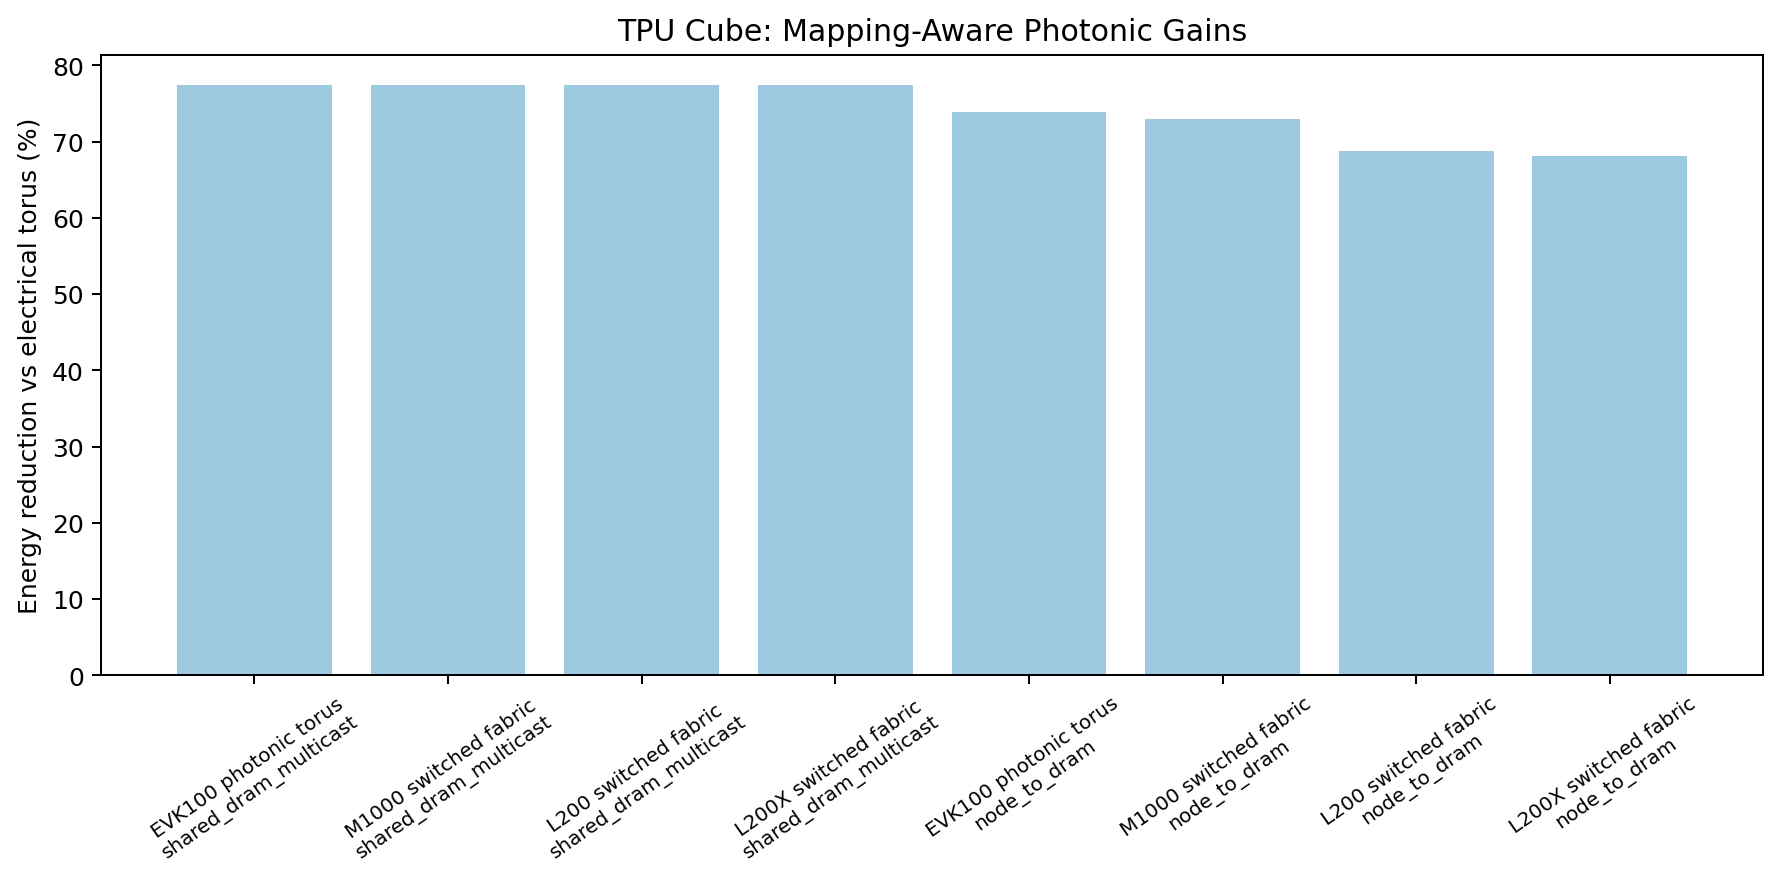
\includegraphics[width=\linewidth]{02_tpu_mapping_reductions.png}\\
\smaller \emph{TPU cube: M1000 multicast removes 99.91\% of network energy.}\\[0.5em]
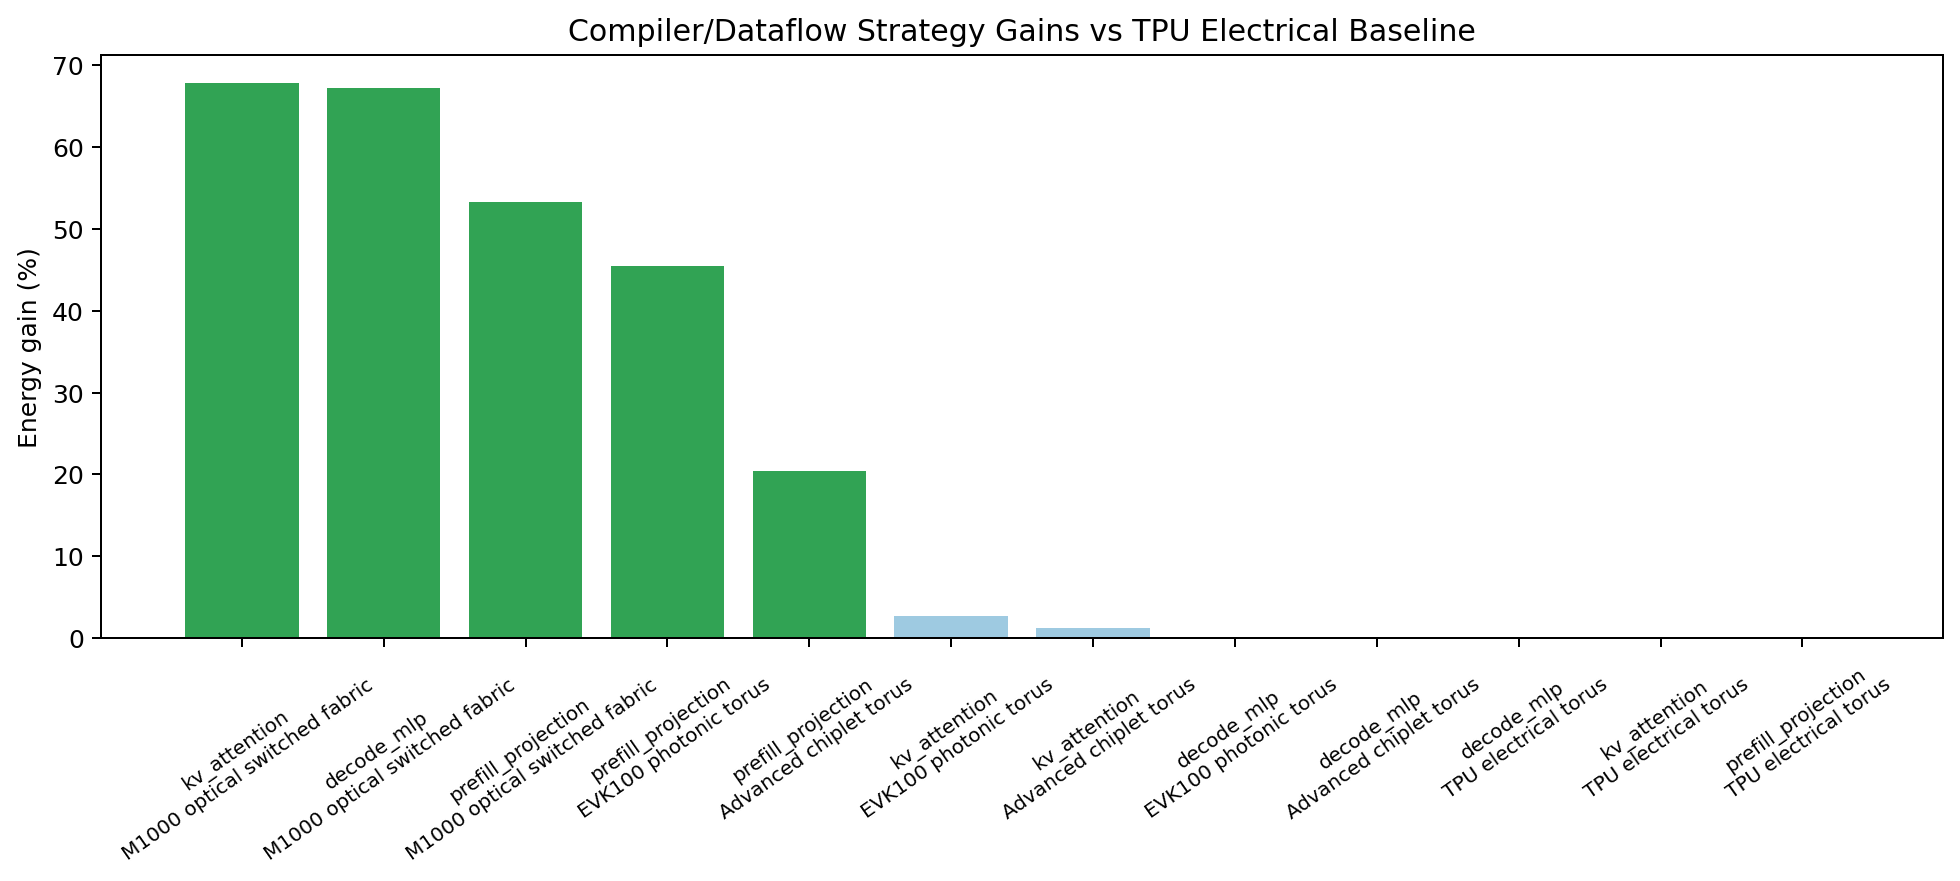
\includegraphics[width=\linewidth]{04_compiler_strategy_choices.png}\\
\smaller \emph{Compiler-visible schedule changes whenever multicast becomes available.}
}

\column{0.34}
\block{5. Superpod}{
\centering
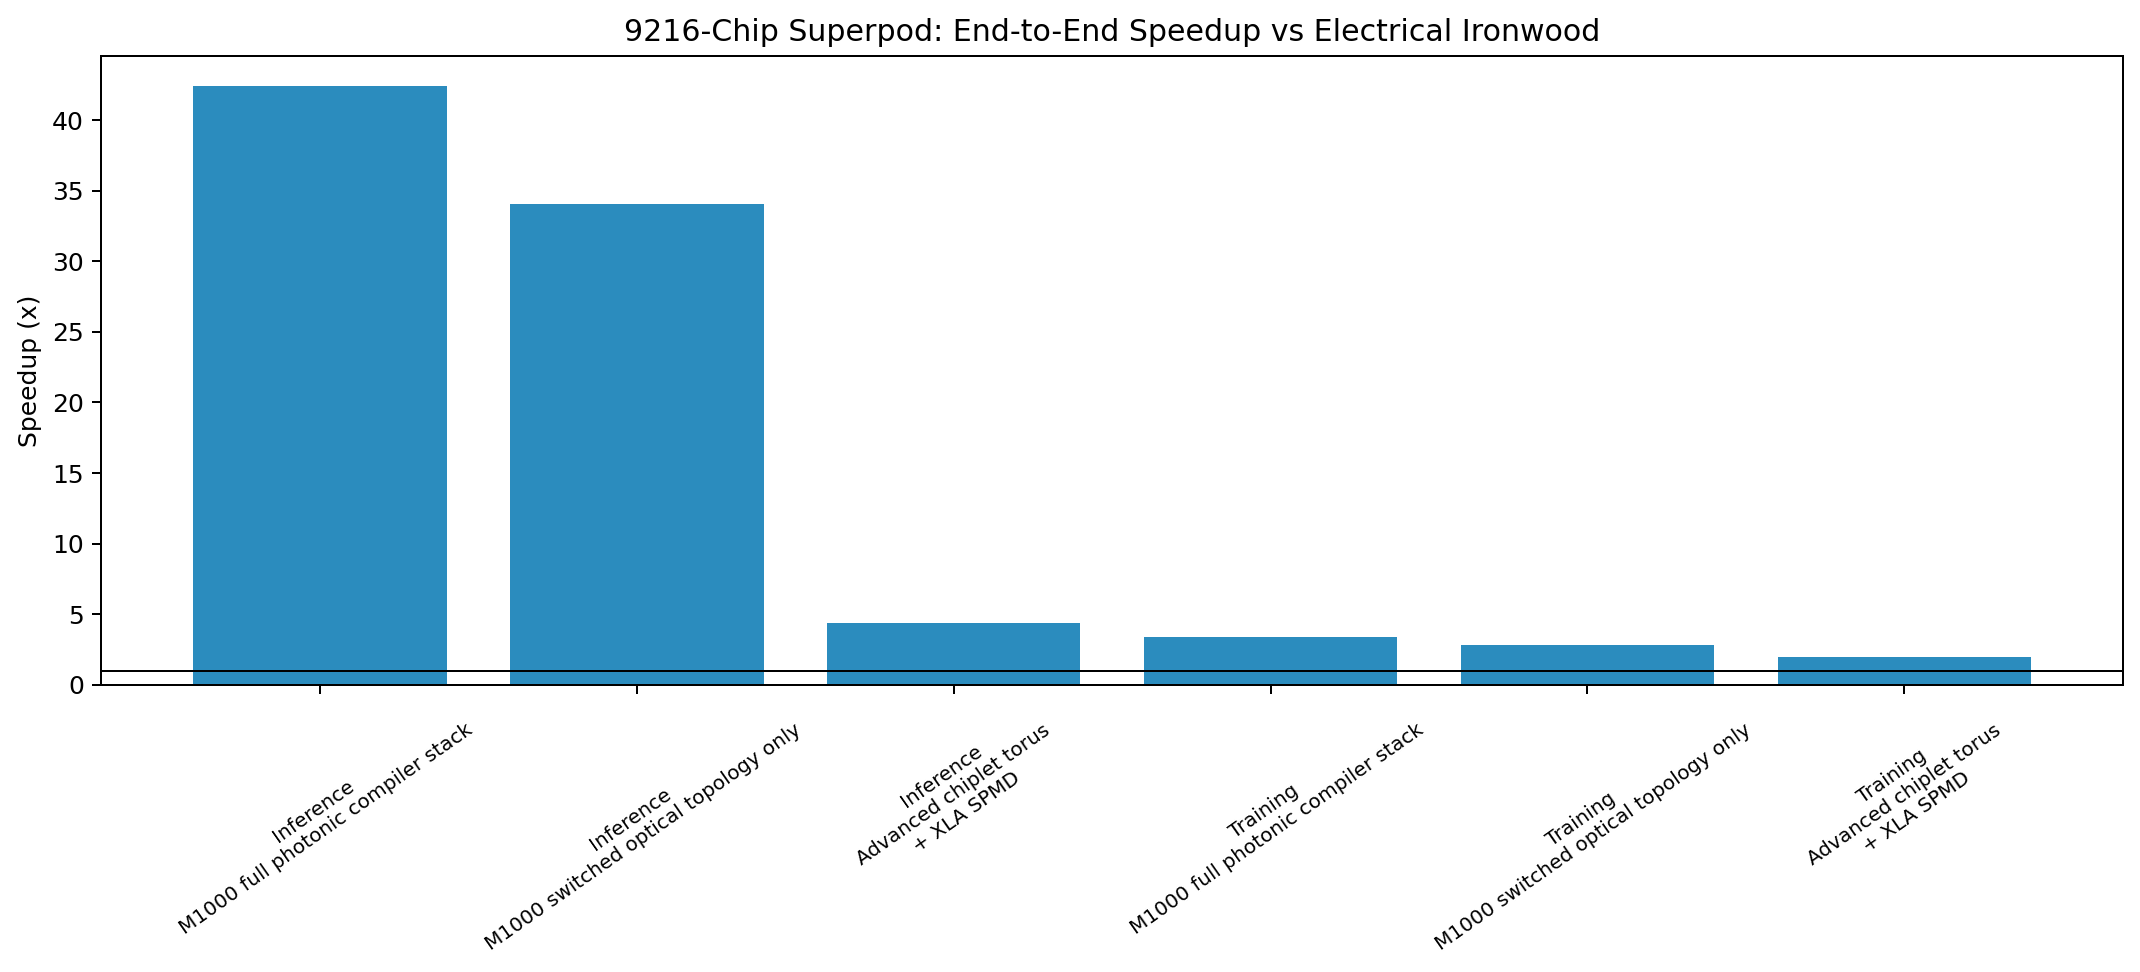
\includegraphics[width=\linewidth]{07_superpod_end_to_end_speedups.png}\\
\smaller \emph{Long-context inference benefits 14.50$\times$; training only 1.43$\times$.}\\[0.5em]
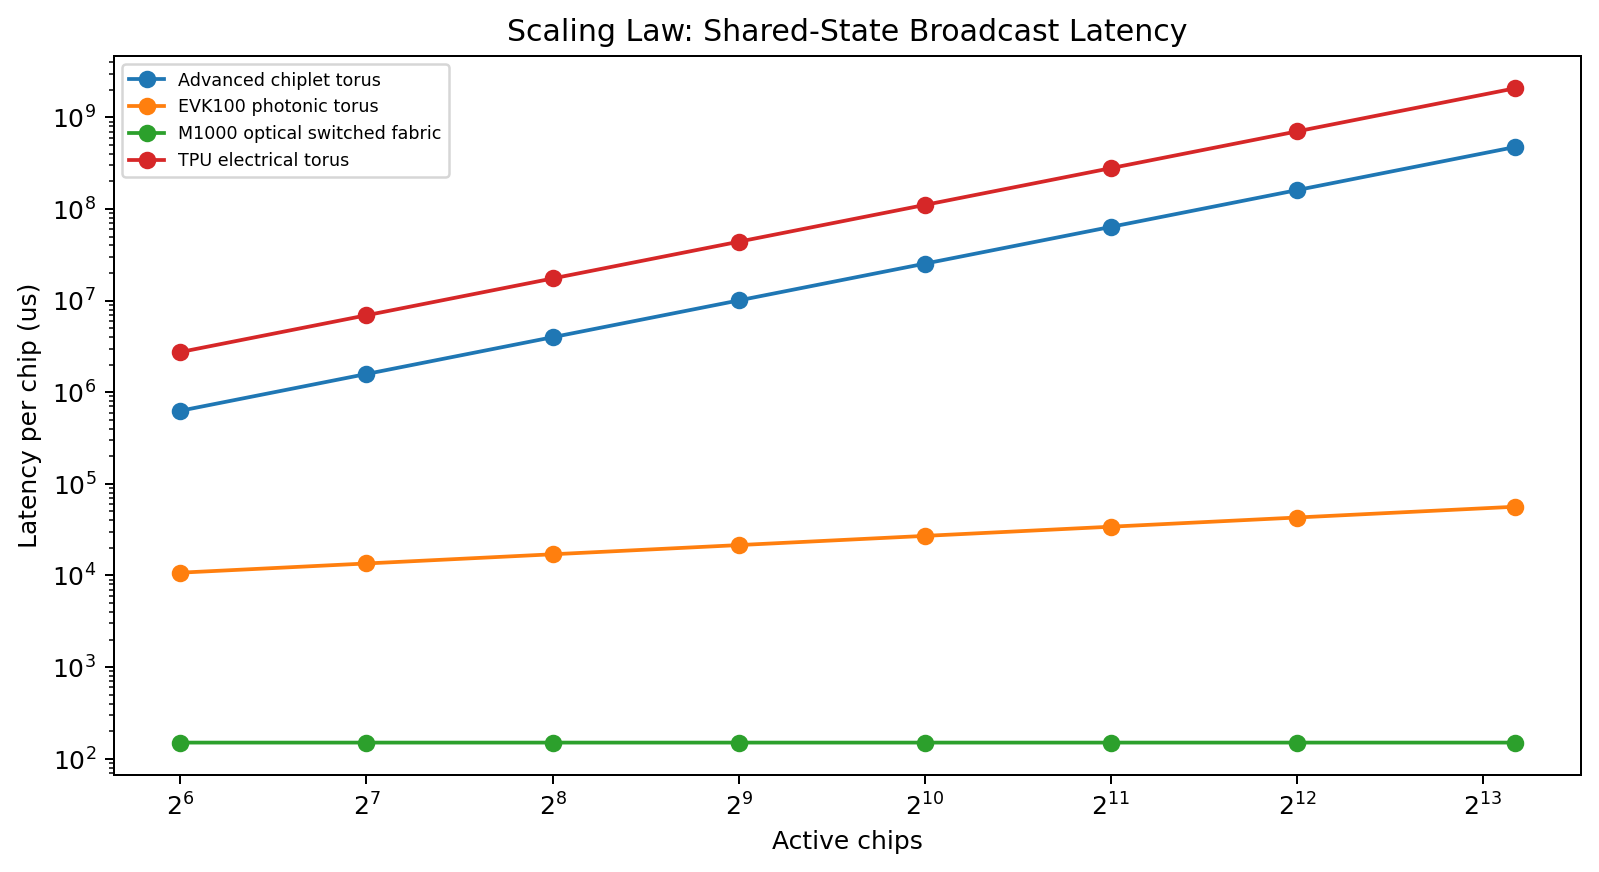
\includegraphics[width=\linewidth]{05_scaling_laws.png}\\
\smaller \emph{Optical multicast scaling exponent stays at 0.00 across 64$\to$9216 chips.}
}
\end{columns}

% Row 3: full-width results
\block{6. Results and Analysis of Results}{
\textbf{Three key insights.}
\begin{enumerate}
\item \textbf{The intra-chip mapping is stable; the distributed
schedule is what changes.} Across 24 (workload, technology, scenario)
cases on the TPU cube, \emph{0/24} inner mapping signatures change.
The benefit lives in layer 4: \emph{5/16} workload--scenario pairs
flip their optimal communication pattern (node-to-node $\to$
shared-DRAM multicast), and the optimal compiler-visible schedule
changes whenever multicast becomes available. Reporting these as
separate layers matches the 6.5930 mapping formalism cleanly. This
is the central conceptual finding.
\item \textbf{Hardware multicast, not raw bandwidth, dominates
shared-state workloads.} The 3.5~\tbps{}, 6~\pjbit{} chiplet
baseline is still beaten by M1000 by \textbf{99.85\%} on shared-DRAM
multicast: $N$ unicasts collapse to one logical broadcast, and
contention disappears on a switched fabric. The same chiplet is
competitive on node-to-node activation exchange.
\item \textbf{Photonics is not a uniform multiplier.} On the
9216-chip superpod, long-context inference reaches
\textbf{14.50}$\times$ speedup; training reaches only
\textbf{1.43}$\times$. Once collectives shrink, training becomes
compute-dominated; inference stays network-exposed because decode and
MoE routing cross the fabric every step. The strong case is
inference and long-context serving, not training payoff.
\end{enumerate}

\begin{minipage}[t]{0.42\linewidth}
\smaller
\begin{tabular}{l r l | l r l}
\toprule
Axis & Value & Setting & Axis & Value & Setting \\
\midrule
16-node energy red.   & 72.21\%        & EVK100 MC          & Compiler best gain    & 67.75\%        & M1000 stream \\
16-node latency red.  & 97.57\%        & EVK100 MC          & Multicast slope       & 0.00           & M1000 64$\to$9216 \\
TPU cube net energy   & 99.91\%        & M1000 MC           & Chiplet vs M1000      & 99.85\%        & MC \\
TPU cube map energy   & 77.70\%        & M1000 KV           & Inference speedup     & 14.50$\times$  & Deep Think \\
Inner maps changed    & 0/24           & cube               & Training speedup      & 1.43$\times$   & Pro MoE \\
Distributed maps      & 5/16           & cluster            & Inference energy      & 51.07\%        & Deep Think \\
\bottomrule
\end{tabular}
\end{minipage}\hfill
\begin{minipage}[t]{0.56\linewidth}
\vspace{-5em}
\textbf{Where it helps.} Long-context inference; sparse-MoE serving;
pooled remote HBM; cache-fill / weight-broadcast traffic.\\[0.4em]
\textbf{Where it does not help.} Local nearest-neighbor exchange
(electrical torus already efficient at one hop); compute-dominated
training stages; mappings already optimal on electrical.\\[0.4em]
\textbf{What worked / did not.} Worked: feedback loop converged in
$\le 3$ iterations; multicast asymmetry as predicted; superpod stage
model reproduced inference-vs-training divergence. Did not work:
encoding the inter-chip NoC as a degenerate \texttt{!Memory} inside
AccelForge produced opaque numbers; we kept the network model
external. The inner mapping signature did not change -- an honest
negative result we report rather than hide.
\end{minipage}
\\[0.4em]
\textbf{Future work.} Direct XLA/Pallas integration; cycle-accurate
optical-switch simulator; co-design of MoE expert placement under
photonic locality; pipeline-parallel + ZeRO-3 training stage model.
}

% Row 4: full-width references
\block{7. References}{
\smaller
[1]~Sze \& Emer, MIT 6.5930 lectures: \emph{Mapping},
\emph{Mapping/Partitioning}, \emph{Advanced Technologies}, Spring 2026.
\quad
[2]~T.~Andrulis et al., ``Architecture-Level Modeling of Photonic DNN
Accelerators,'' ISPASS 2024.
\quad
[3]~Lightmatter, Passage product family / EVK50 / EVK100 / L200 /
L200X / M1000 product pages and SC25 \& ISES 2025 talks
(\texttt{lightmatter.co}).
\quad
[4]~Google Cloud, ``TPU v5p,'' ``Cloud TPU7x'' (Apr.~2026), and
``Inside the Ironwood TPU co-designed AI stack''; P. Kanwar, ``TPU
Rack Scale Systems,'' Hot Chips 2025 Tutorial.
\quad
[5]~PyTorch/XLA, ``SPMD user guide.''
\quad
[6]~Google, ``Gemini 3'' (Nov.~2025), ``Gemini 3 Deep Think''
(Feb.~2026).
}

\end{document}
